\section{Өгөгдлийн сангийн диаграм}
\begin{figure}[ht]
  \centering
  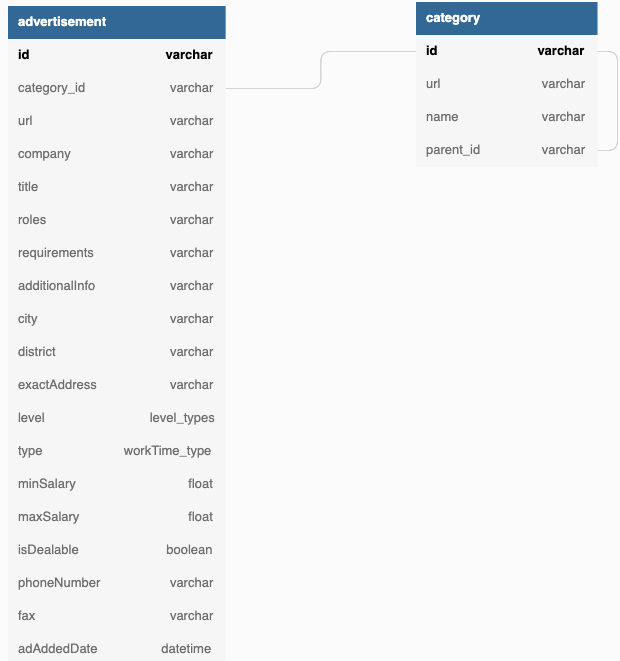
\includegraphics[width = \textwidth]{images/dbDiagram.png}
  \caption{Өгөгдлийн сангийн диаграм}\label{fig:dbDiagram}
\end{figure}
\newpage

\section{Өгөгдлийн элемент}
Чатбот системийн өгөгдлийн сангийн диаграмд харуулсан хүснэгтүүдэд агуулагдах мэдээлэл болон үүргийн талаар дэлгэрэнгүй тайлбарласан болно. 
\subsection{advertisement - Ажлын байрны зар}
Ажлын байрны зар нь ямар категори буюу ангилалд, ямар холбоо барих хаягийн хамтаар хадгалагдаж буй мэдээлэл болон бусад дэлгэрэнгүй мэдээллийг харуулсан байна. 
\begin{table}[ht]
  \caption{advertisement хүснэгт}\label{table:advertisement1}
  \begin{tabular}{|l|l|c|c|c|l|}
    \hline
    \multicolumn{1}{|c|}{\textbf{№}} & \multicolumn{1}{c|}{\textbf{Баганын нэр}} & \textbf{\begin{tabular}[c]{@{}c@{}}Түлхүүр \\ өгөгдөл\end{tabular}} & \textbf{\begin{tabular}[c]{@{}c@{}}Өгөгдлийн \\ төрөл\end{tabular}} & \textbf{\begin{tabular}[c]{@{}c@{}}Хоосон \\ утга\end{tabular}} & \multicolumn{1}{c|}{\textbf{Тайлбар}}                                                             \\ \hline
    1                                & \textbf{id}                               & PK                                                                  & varchar                                                             & not null                                                        & \begin{tabular}[c]{@{}l@{}}Ажлын байрны зарын дахин \\ давтагдашгүй дугаар\end{tabular}           \\ \hline
    2                                & category\_id                              & FK                                                                  & varchar                                                             & not null                                                        & \begin{tabular}[c]{@{}l@{}}Ажлын байрны зард хамаарах \\ ангиллын дугаар\end{tabular}            \\ \hline
    3                                & url                                       &                                                                     & varchar                                                             & not null                                                        & Ажлын байрны зарын хаяг                                                                           \\ \hline
    4                                & company                                   &                                                                     & varchar                                                             & not null                                                        & Ажил олгогч компани / хүн                                                                         \\ \hline
    5                                & title                                     &                                                                     & varchar                                                             & not null                                                        & Ажлын зарын гарчиг                                                                                \\ \hline
    6                                & roles                                     &                                                                     & varchar                                                             & null                                                            & Гүйцэтгэхүндсэн үүрэг                                                                             \\ \hline
    7                                & requirements                              &                                                                     & varchar                                                             & null                                                            & \begin{tabular}[c]{@{}l@{}}Ажлын байранд тавигдах \\ шаардлага\end{tabular}                       \\ \hline
    8                                & additionalInfo                            &                                                                     & varchar                                                             & null                                                            & Нэмэлт мэдээлэл                                                                                   \\ \hline
    9                                & location\_id                              & FK                                                                  & varchar                                                             & not null                                                        & \begin{tabular}[c]{@{}l@{}}Ажлын байрны зард хамаарах \\ ангиллын дугаар\end{tabular}            \\ \hline
    10                               & level                                     &                                                                     & level\_types                                                        & null                                                            & Ажлын түвшин                                                                                      \\ \hline
    11                               & type                                      &                                                                     & workTime\_type                                                      & null                                                            & Ажиллах цагийн төрөл                                                                              \\ \hline
    % 12                               & minSalary                                 &                                                                     & float                                                               & null                                                            & Доод цалин                                                                                        \\ \hline
    % 13                               & maxSalary                                 &                                                                     & float                                                               & null                                                            & Дээд цалин                                                                                        \\ \hline
    % 14                               & isDealable                                &                                                                     & boolean                                                             & null                                                            & Тохиролцох эсэх                                                                                   \\ \hline
    % 15                               & contact\_id                               & FK                                                                  & varchar                                                             & not null                                                        & \begin{tabular}[c]{@{}l@{}}Ажлын байрны зард хамаарах \\ холбоо барих хаягийн дугаар\end{tabular} \\ \hline
    % 16                               & adAddedDate                               &                                                                     & datetime                                                            & not null                                                        & Зар нийтэлсэн огноо                                                                               \\ \hline
    \end{tabular}
\end{table}
\begin{table}[ht]
    \begin{tabular}{|l|l|c|c|c|l|}
      \hline
      \multicolumn{1}{|c|}{\textbf{№}} & \multicolumn{1}{c|}{\textbf{Баганын нэр}} & \textbf{\begin{tabular}[c]{@{}c@{}}Түлхүүр \\ өгөгдөл\end{tabular}} & \textbf{\begin{tabular}[c]{@{}c@{}}Өгөгдлийн \\ төрөл\end{tabular}} & \textbf{\begin{tabular}[c]{@{}c@{}}Хоосон \\ утга\end{tabular}} & \multicolumn{1}{c|}{\textbf{Тайлбар}}                                                             \\ \hline
      12                               & minSalary                                 &                                                                     & float                                                               & null                                                            & Доод цалин                                                                                        \\ \hline
      13                               & maxSalary                                 &                                                                     & float                                                               & null                                                            & Дээд цалин                                                                                        \\ \hline
      14                               & isDealable                                &                                                                     & boolean                                                             & null                                                            & Тохиролцох эсэх                                                                                   \\ \hline
      15                               & contact\_id                               & FK                                                                  & varchar                                                             & not null                                                        & \begin{tabular}[c]{@{}l@{}}Ажлын байрны зард хамаарах \\ холбоо барих хаягийн дугаар\end{tabular} \\ \hline
      16                               & adAddedDate                               &                                                                     & datetime                                                            & not null                                                        & Зар нийтэлсэн огноо                                                                               \\ \hline
      \end{tabular}
\end{table}
\\Энд \textit{level} буюу ажлын түвшин, \textit{type} буюу ажлын цагийн өгөгдлийн төрлийг тодорхойлохдоо дараах байдлаар зааж өгсөн.
\\\textbf{Enum level\_types} буюу ажлын түвшний шаардлага нь дараах үндсэн 4 өгөгдлийн төрлөөс хамаарна:
\begin{itemize}
  \item student - Оюутан / дадлагажигч
  \item professional - Мэргэжлийн
  \item occupasionDoesntRequire - Мэргэжил шаардахгүй
  \item intermediateManagemet - Дунд шатны удирдлага
\end{itemize}
\textbf{workTime\_type} буюу ажиллах цагийн нөхцөл нь дараах үндсэн 4 өгөгдлийн төрлөөс хамаарна:
\begin{itemize}
  \item shift - Ээлжийн
  \item fullTime - Бүтэн цагийн
  \item halfTime - Хагас цагийн
  \item contract - Гэрээт / зөвлөх
\end{itemize}

\subsection{category - Ангилал}
Ажлын байрны зарын бүх ангиллуудын хаяг болон нэрийн мэдээллийг хадгалах хүснэгт юм. Ангиллууд нь дэд ангилал байж болох учир түүнийг эцэг ангиллын дугаарыг хадгалах байдлаар зохиомжлов. 
\begin{table}[ht]
  \caption{category хүснэгт}\label{table:category}
  \begin{tabular}{|l|l|c|l|c|l|}
  \hline
  \multicolumn{1}{|c|}{\textbf{№}} & \multicolumn{1}{c|}{\textbf{Баганын нэр}} & \textbf{\begin{tabular}[c]{@{}c@{}}Түлхүүр\\ өгөгдөл\end{tabular}} & \multicolumn{1}{c|}{\textbf{\begin{tabular}[c]{@{}c@{}}Өгөгдлийн\\ төрөл\end{tabular}}} & \textbf{\begin{tabular}[c]{@{}c@{}}Хоосон\\ Утга\end{tabular}} & \multicolumn{1}{c|}{\textbf{Тайлбар}}                                   \\ \hline
  1                                & \textbf{id}                               & PK                                                                 & varchar                                                                                 & not null                                                       & \begin{tabular}[c]{@{}l@{}}Ажлын байрны зарын\\ ангиллын дугаар\end{tabular} \\ \hline
  2                                & url                                       &                                                                    & varchar                                                                                 & not null                                                       & Ангиллын хаяг                                                          \\ \hline
  3                                & name                                      &                                                                    & varchar                                                                                 & not null                                                        & Ангиллын нэр                                                           \\ \hline
  4                                & parent\_id                                & FK                                                                 & varchar                                                                                 & null                                                           & Эцэг ангиллын дугаар                                                   \\ \hline
  \end{tabular}
\end{table}
\subsection{location - Байршил}
Ажлын байрны байршил болон хот, аймаг, дүүргийн дэлгэрэнгүй өгөгдлийг хадгална. 
\begin{table}[ht]
  \caption{location хүснэгт}\label{table:location1}
  \begin{tabular}{|l|l|c|l|c|l|}
  \hline
  \multicolumn{1}{|c|}{\textbf{№}} & \multicolumn{1}{c|}{\textbf{Баганын нэр}} & \textbf{\begin{tabular}[c]{@{}c@{}}Түлхүүр\\ өгөгдөл\end{tabular}} & \multicolumn{1}{c|}{\textbf{\begin{tabular}[c]{@{}c@{}}Өгөгдлийн\\ төрөл\end{tabular}}} & \textbf{\begin{tabular}[c]{@{}c@{}}Хоосон\\ Утга\end{tabular}} & \multicolumn{1}{c|}{\textbf{Тайлбар}}                                                  \\ \hline
  1                                & \textbf{id}                               & PK                                                                 & varchar                                                                                 & not null                                                       & \begin{tabular}[c]{@{}l@{}}Ажлын байрны зарын \\ хаягийн дугаар\end{tabular}           \\ \hline
  2                                & city                                      &                                                                    & varchar                                                                                 & null                                                           & \begin{tabular}[c]{@{}l@{}}Ажлын байрны зарын байрших\\ хот, аймгийн нэр\end{tabular}  \\ \hline
  \end{tabular}
\end{table}
\begin{table}[ht]
    \begin{tabular}{|l|l|c|l|c|l|}
    \hline
    \multicolumn{1}{|c|}{\textbf{№}} & \multicolumn{1}{c|}{\textbf{Баганын нэр}} & \textbf{\begin{tabular}[c]{@{}c@{}}Түлхүүр\\ өгөгдөл\end{tabular}} & \multicolumn{1}{c|}{\textbf{\begin{tabular}[c]{@{}c@{}}Өгөгдлийн\\ төрөл\end{tabular}}} & \textbf{\begin{tabular}[c]{@{}c@{}}Хоосон\\ Утга\end{tabular}} & \multicolumn{1}{c|}{\textbf{Тайлбар}}                                                  \\ \hline
    3                                & district                                  &                                                                    & varchar                                                                                 & null                                                           & \begin{tabular}[c]{@{}l@{}}Ажлын байрны зарын байрших\\ дүүрэг, сумын нэр\end{tabular} \\ \hline
    4                                & exactAddress                              &                                                                    & varchar                                                                                 & null                                                           & Дэлгэрэнгүй хаяг                                                                       \\ \hline
    \end{tabular}
\end{table}
\subsection{contactInfo - Холбоо барих}
Ажлын байр олгогчийн хаягийн дэлгэрэнгүй өгөгдлийг хадгалана.
\begin{table}[ht]
  \caption{contactInfo хүснэгт}\label{table:contactInfo}
  \begin{tabular}{|l|l|c|l|c|l|}
  \hline
  \multicolumn{1}{|c|}{\textbf{№}} & \multicolumn{1}{c|}{\textbf{Баганын нэр}} & \textbf{\begin{tabular}[c]{@{}c@{}}Түлхүүр\\ өгөгдөл\end{tabular}} & \multicolumn{1}{c|}{\textbf{\begin{tabular}[c]{@{}c@{}}Өгөгдлийн\\ төрөл\end{tabular}}} & \textbf{\begin{tabular}[c]{@{}c@{}}Хоосон\\ Утга\end{tabular}} & \multicolumn{1}{c|}{\textbf{Тайлбар}}                                                \\ \hline
  1                                & \textbf{id}                               & PK                                                                 & varchar                                                                                 & not null                                                       & \begin{tabular}[c]{@{}l@{}}Ажил олгогчтой холбоо барих\\ хаягийн дугаар\end{tabular} \\ \hline
  2                                & phoneNumber                               &                                                                    & int                                                                                     & null                                                           & Ажил олгогчийн утасны дугаар                                                         \\ \hline
  3                                & fax                                       &                                                                    & int                                                                                     & null                                                           & Ажил олгогчийн факс дугаар                                                           \\ \hline
  \end{tabular}
  \end{table}

\section{Өгөгдлийн сангийн холбоосын тайлбар}
\begin{itemize}
  \item Нэг ангилал буюу категорид олон ажлын байрны зар байж болно.
  \item Нэг ангилал буюу категорид олон категори байж болно. 
  \item Нэг ажлын байрны зард нэг байршлын мэдээлэл байна.
  \item Нэг ажлын байрны зард нэг холбоо барих хаягийн мэдээлэл байна.
\end{itemize}